\documentclass[journal,transmag]{IEEEtran}
%
% If IEEEtran.cls has not been installed into the LaTeX system files,
% manually specify the path to it like:
% \documentclass[journal]{../sty/IEEEtran}
\usepackage{amsthm}
\usepackage{graphicx}
\usepackage{algorithm}
\usepackage{cite}



\ifCLASSINFOpdf
  % \usepackage[pdftex]{graphicx}
  % declare the path(s) where your graphic files are
  % \graphicspath{{../pdf/}{../jpeg/}}
  % and their extensions so you won't have to specify these with
  % every instance of \includegraphics
  % \DeclareGraphicsExtensions{.pdf,.jpeg,.png}
\else
  % or other class option (dvipsone, dvipdf, if not using dvips). graphicx
  % will default to the driver specified in the system graphics.cfg if no
  % driver is specified.
  % \usepackage[dvips]{graphicx}
  % declare the path(s) where your graphic files are
  % \graphicspath{{../eps/}}
  % and their extensions so you won't have to specify these with
  % every instance of \includegraphics
  % \DeclareGraphicsExtensions{.eps}
\fi



\hyphenation{op-tical net-works semi-conduc-tor}

\begin{document}

\title{Bisic Implementation of Sparse Fourier Transform}

\author{\IEEEauthorblockN{Shi Wang,
Yi Han,
Xiaoran Fan
}}

\markboth{REPORT OF 332:521 DIGITAL SIGNALS AND FILTER TERM PROJECT, 2015 FALL}%
{Shell \MakeLowercase{\textit{et al.}}: Bare Demo of IEEEtran.cls for IEEE Transactions on Magnetics Journals}

\IEEEtitleabstractindextext{%
\begin{abstract}
The Sparse Fast Fourier Transform is a recent algorithm developed by Hassanieh et al. at MIT for Discrete Fourier Transforms on signals with a sparse frequency domain. In this report we illustrated the basic theory of sparse Fourier transform and a simple implementation. And we tried different searching methods in our implementation. We compared the running time of our SFT and FFT later. And applied different signal to noise level noise onto our generated signal to test the robustness of our implementation. We also compared the running time of each stage in our paper. Though our implementation is not as fast as the Matlab built-in FFT, there are a lot of stages could be optimized. Finally we discussed some issues in implementing this algorithm for our future work.
\end{abstract}

% Note that keywords are not normally used for peerreview papers.
\begin{IEEEkeywords}
signal processing, sparse fourier transform, FFT.
\end{IEEEkeywords}}



% make the title area
\maketitle


% To allow for easy dual compilation without having to reenter the
% abstract/keywords data, the \IEEEtitleabstractindextext text will
% not be used in maketitle, but will appear (i.e., to be "transported")
% here as \IEEEdisplaynontitleabstractindextext when the compsoc 
% or transmag modes are not selected <OR> if conference mode is selected 
% - because all conference papers position the abstract like regular
% papers do.
\IEEEdisplaynontitleabstractindextext
% \IEEEdisplaynontitleabstractindextext has no effect when using
% compsoc or transmag under a non-conference mode.







% For peer review papers, you can put extra information on the cover
% page as needed:
% \ifCLASSOPTIONpeerreview
% \begin{center} \bfseries EDICS Category: 3-BBND \end{center}
% \fi
%
% For peerreview papers, this IEEEtran command inserts a page break and
% creates the second title. It will be ignored for other modes.
\IEEEpeerreviewmaketitle

\theoremstyle{plain}
\newtheorem{thm}{Theorem}[section] % reset theorem numbering for each chapter

\theoremstyle{definition}
\newtheorem{defn}[thm]{Definition} % definition numbers are dependent on theorem numbers
\newtheorem{exmp}[thm]{Example}

\section{Introduction}
% The very first letter is a 2 line initial drop letter followed
% by the rest of the first word in caps.
% 
% form to use if the first word consists of a single letter:
% \IEEEPARstart{A}{demo} file is ....
% 
% form to use if you need the single drop letter followed by
% normal text (unknown if ever used by the IEEE):
% \IEEEPARstart{A}{}demo file is ....
% 
% Some journals put the first two words in caps:
% \IEEEPARstart{T}{his demo} file is ....
% 
% Here we have the typical use of a "T" for an initial drop letter
% and "HIS" in caps to complete the first word.


\subsection{Motivation}

the Discrete Fourier Transform is the most important technique in digital signal processing, it makes processing signal with digital equipments possible, which significantly improved the reliability and efficiency of signal processing systems. However, the direct way of computing the DFT require $O(N^2)$ time, as the signal length increase, this time could be relatively large, it’s a common thing nowadays, lots of useful applications of signal processing are dealing with signals with incredibly large size, it’s almost impossible to directly use the DFT formula. 

The Fast Fourier Transform is one of, and is the most popular and fundamental numerical algorithm to compute the DFT, it is much faster, the computational complexity is $O(N\log N)$ time. The algorithm play an central role in several application areas, including signal processing, audio/image/video compression. However, facing the big data problems of these days, the number nlogn can also be too large in applications, thus, people seek to find faster ways to compute DFT in some specific situations, the Sparse Fourier Transform is one of the successful algorithm of this kind.

The SFT deals with the situation when most of the spectrum of the signal is zero or close to zero, with only a small number of frequency coefficients being large, the spectrum is consider to be sparse, this is common in audio/image/video signals\cite{chandrakasan1996data}, it also has applications in compressed sensing\cite{donoho2006compressed,candes2006robust} and spectrum sensing\cite{lin2011new}. 


% needed in second column of first page if using \IEEEpubid
%\IEEEpubidadjcol

\subsection{Related Work}
First such algorithm(Hadamard transform) appeared on [KM91], After then many research group worked on the algorithm, e.g. Gilbert’s group from MSU\cite{gilbert2005improved,gilbert2008tutorial}, and Hassanieh’s group from MIT, other contributors includes Iwen from UMN\cite{iwen2010combinatorial}.

Most popular variants of this kind can be classified into two categories, to iterate\cite{gilbert2005improved} or not to iterate\cite{hassanieh2012simple}. both categories apply filter design technique to isolate each dominant frequency and then doing single frequency recovery to find the location and magnitude of them, in order to do the filtering in sublinear time, the n-dimensional filter vector $G$ tis supposed to be concentrated both in time and frequency, that is, $G$ is zero except at a small number of time coordinates, and its Fourier transform $\hat{G}$ is negligible except at a small fraction $O(1/k)$ of the frequency coordinates. However, since iteration-based methods use filters with slow out-passband decay, two adjacent window will leak into each other, which will affect the single frequency recovery process, to solve this problem, it pick the frequency with largest magnitude in the bin, and at the end of each iteration, subtract the detected frequencies, doing the same process on the remaining signal, as the iteration loops, the spectrum of the signal becomes sparser, so it is more likely to identify all the dominant frequencies. However, subtracting detected coefficients at the end of each iteration loop is somewhat time consuming, Hassanieh et al introduced a way\cite{hassanieh2012nearly} of directly subtract identified coefficients directly from the bins,  since each of the coefficient “falls” into only one bin, the operation can be done in linear time. Moreover, In the paper, they also developed a block recovery technique to improved computational efficiency, instead of recover bit by bit, they recover the index one block at a time. 

The other category of methods do not require subtraction and iteration, however, in the inner stage they do have iteration loops. these methods use ideal filter to isolate frequencies, thus don’t have leakage problems, however, they require the length of the signal can be divided by the length of the filters. as mentioned above, these methods have inner loops on identification and estimation stage, in order to find the most suitable frequencies and their magnitude as well as improve the stability. Note that since these inner loops are independent of each other, parallel computing technique can be apply to further improve efficiency.


\subsection{Our Frame}
In this paper we considered a simple and basic implementation of SFT, evaluated some of its properties against FFT, and proposed some challengings that might be improved in further studies.

Suppose we have a sparse signal with length $N$ and sparsity $k$, that is to say, among all $N$ point frequencies on $k$ of them are non-zero, the task is to identify all of them are estimate their magnitudes. As mentioned above, we designed a filter which is highly concentrated both in time and frequency domain in order to reduce the time required for convolution. We shifted the filter by multiplying a set of phase factors in the time domain to cover the whole range of the spectrum, in this way we get a set of filters(filter bank), each of which “picks” a small fraction of the frequency range, the process is called binning or shattering. If the non-zero frequencies of the signal is separated enough, it is very likely that each bin contains only one of such frequencies. This is guaranteed by applying a permutation method to the original signal\cite{hassanieh2012simple}, that is, permuting samples the time domain and changing their phases, later we can see that such manipulations actually permute the frequency points of the signal. The permuted spectrum is likely to “looks” uniformly distributed, with dominant frequencies well separated, thus those frequencies is more likely to be isolated. however, even if more than one dominant frequencies appeared in the same bin, we simple pick up the one with largest magnitude, later iterations will guarantee that all the dominant frequencies can be detected. Also in later sections we can see that such permutation process is reversible, thus after dominant frequencies are identified, we can recover the original location of them, therefore recover the original signal spectrum.

After binning the signal spectrum, single frequency recovery techniques is applied to identify the dominant frequency in the bins. we applied three of such techniques, phase encoding, an aliasing-based search method, and binary search. Phase encoding utilized the relation of phase factors of two adjacent time samples, however, it is sensitive to noise; The core idea, or the basis of the aliasing-based search method is the Chinese Reminders Theorem, which guarantee that congruence equations derived from subsampled DFT by a set of co-prime numbers have unique solution in the range of $N$ if product of the co-prime numbers are greater than $N$. The binary search method divide the complex plane into four parts, and compare the desired frequency with four points on the axis and the unit circle to narrow it range, by applying such process several time, the location of the desired frequency can be figured out. After identifying the dominant frequency locations, doing remapping we can obtain the index of these frequencies in the original signal, next step is to estimate the magnitude, or coefficient of these frequencies. To make our algorithm efficient, we computed a subsampled version of DFT, by randomly pick a small number of uniformly distributed samples. We evaluated the influence of changing number of samples on the stability of the estimator. Note that for the aliasing-based method, the subsampled DFT have already been computed in the identification stage.

We do the whole process above several times to avoid situation when multiple dominant frequencies appear in the same bins to improve the stability of the algorithm. At the end of each loop we subtract identified frequencies from the original signal, this makes the new signal sparser.

Then remaining content of the paper are organized as follows: In section 2, we describe each step of the algorithm in detail; Next in section 3, We evaluate the runtime of our implementation against MATLAB built-in FFT when the signal size and sparsity change, as well as the stability of the algorithm when noise is added. Finally in section 4, we draw our conclusions and propose some challengings that might be improved in further studies.

flow chart requried

\section{The Algorithm}
\subsection{Permutation}
As mentioned in Introduction, a binning, or shuttering method is introduced to isolated each single dominant frequency point, this can be down by apply a set of shifted filters $G$, or a filter bank  to the signal. However, such method require dominant frequencies of the signal not to be close to each other, or in other words, not  collide with each other, We can’t guarantee a signal to have this property. In order to feed the filter bank with such a signal with well separated spectrum, a pseudo-random permutation method is introduced\cite{hassanieh2012simple}. The permutation method scales and circular shifts the time indices, to obtain a permuted version of the original spectrum, the permuted spectrum “looks” uniformly distributed, the each of the dominant frequency is high possible to isolated. 

\begin{defn}
	Define a transform $P_{\sigma,\tau}$, for any vector of length $N$, an random integer $\sigma\in[N]$, gcd($\sigma,N$) = 1 mod $N$  and an integer $\tau\in[N]$, if time domain indices $i$ is mapped to $\sigma i+\tau$, or $(P_{\sigma,\tau}x)_i = x_{\sigma i+\tau}$, then in the frequency domain
	\begin{equation}
		\widehat{(P_{\sigma,\tau}x)}_{\sigma i}=\hat{x}_i\omega^{-\tau i}.
		\label{eq1}
	\end{equation} 
\end{defn}

\begin{proof}
	For any time index $a$, $\widehat{(P_{\sigma,\tau}x)}_a=\sum_{j=1}^{n}x_{\sigma j+\tau}\omega^{\sigma j}=\sum_{j=1}^{n}x_j\omega^{a(j-\tau)\sigma^{-1}}=\hat{x}_{a\sigma^{-1}}\omega^{-\tau a\sigma^{-1}}$.
\end{proof}

\begin{figure}[htbp]
	\includegraphics[width=0.5\textwidth]{permutation}
	\caption{Example of the permutation process.}
	\label{permutation}
\end{figure}

Figure (\ref{permutation})  shows an example of the permutation process, as we can see, the dominant frequencies are separated enough.

In order to recover the original indices of the dominant frequencies, the permutation should be reversible, this can be easily seen from Equation (\ref{eq1}), $\hat{x_{i}}=\hat{x}_{\sigma i}^{\prime}\omega^{\tau i}$. Note that in order to find $\sigma^{-1}$, $\sigma$ should be a co-prime of $N$.




\subsection{Binning}
As mentioned in the previous section, After permutation the spectrum, dominant frequencies are more likely to be separated when pass throuth a set of filters, here we present our idea and thinking of the process.

The basic idea is simple, suppose we have a lowpass filter $h[n]$ with cut-off frequency $\frac{N}{k}$, $k$ is the number of filters we want to have(note that here k is different from the sparsity of signal), in order to obtain the set of filters, we simply multiple a set of phase factors to the lowpass filter, which result in frquency shift in the frequency domain
\begin{equation}
h_k[n]=h[n]\omega^k, \quad k = 1,2,...,N.
\end{equation}
\begin{figure}[htbp]
	\includegraphics[width=0.5\textwidth]{bins}
	\caption{unifomly distributed frequency points are separated into different bins.}
	\label{bins}
\end{figure}
For basic realization of the idea, we simply used a ideal lowpass filter with passband coefficients 1 and other coefficients 0; We apply the signal to the filterbank, as shown in Figure (\ref{bins}), most dominant frequencies have been separated. In order to improve stability, we choose number of filters to be larger than the sparsity of the signal, thus some of the bins will have no dominant frequencies at all, to distinguish such bins before the single frequency recovery stage, we compute the energy of each bin in time domain. Bins with dominant frequency and bins without are different in energy, according to the Paserval's Theorem, such difference is reflected in the time domain, by computing the energy of the original signal in time domain and set a threshold according to value, we can distinguish these two patterns of bins. In the ideal case which noise is not involved, the threshold works perfectly, however, when noise is added to the signal, it started to fall, and the proper threshold varies as the SNR of noise changes. Anyway, the two patterns remains distinguished, some pattern recognition technique can be introduced to find  adaptive thresholds.

However, time domain sequences of such ideal filters is not concentrated, values are distributed all over the range $N$, in this case, computational efficiency cannot be guaranteed, convolution with such kind of filters is time comsumin, in fact only the binning stage have a computational complexity of $O(N^2)$.

In order to make the algorithm sublinear, the filter should be both concentrated in time and frequency domain, although ideal lowpass filter can be concentrated in frequency domain, it is fully occupied in time domain, refence literatures mentioned about convolving the ideal filter with a Gaussian window or Dolph-CHebyshev window\cite{hassanieh2012simple}, dragging the tail of the filter in frequency domain will result in highly decayed sidelobe magnitude. However, too long tail will cause serious leakage problems, thus it's a trade-off.

\subsection{Single Frequency Recovery}
After binning the dominant frequencies, single frequency recovery techniques are applied to bins that are likely to have frequency with large coefficient. We implement three of such methods.
\subsubsection{Phase Encoding}

It is the simplest way to find the frequency index. If the sequence only has one frequency, We can obtain $\omega_0$ by choosing a random number between 0 and $N-1$ and compute
\begin{equation}
	\frac{\arctan \frac{imag(s_k[i+1]/s_k[i])}{real(s_k[i+1]/s_k[i])}}{2\pi}\: mod \: N,
\end{equation}
if $real(s_k[i+1]/s_k[i])$, we compute
\begin{equation}
	(\frac{\arctan \frac{imag(s_k[i+1]/s_k[i])}{real(s_k[i+1]/s_k[i])}}{2\pi}+\frac{N}{2})\: mod \: N. 
\end{equation}
The method is very efficient since it only used two of the signal samples, however, it is very sensitive to noise, when noise is added to the coefficients, simply dividing two adjacent frequency coefficients will lead to wrong result.

\subsubsection{An Aliasing-based Method}
First,we compute the inverse DFT of $f_n$
\begin{equation}
	f_n = \sum_{k}^{N-1}\hat{f}_ke^{j\frac{2\pi}{N}nk}
	\label{inv}
\end{equation} 
Second, we downsample $f_n$ by $m$
\begin{equation}
	a_n=f_{mn} \quad n=0,1,2,...,m-1
	\label{dow}
\end{equation}
Third, we compute the $\frac{N}{m}$-point DFT of $a_n$
\begin{equation}
	\hat{a}_k = \sum_{n=0}^{N/k}a_ne^{-j\frac{2\pi}{N/m}nk} \quad k = 0,1,2,...,m-1
	\label{dft}
\end{equation}
Finally, by substituting (\ref{inv}), (\ref{dow}) to (\ref{dft}) we get
\begin{equation}
	\hat{a}_k=\sum_{n=0}^{m-1}\hat{f}_{\frac{N}{k}n+k}
	\label{rel}
\end{equation}
From Equation (\ref{rel}) we can see that if we downsample the filtered signal by $m$, then compute $\frac{N}{m}$-point DFT, the new Fourier coefficients $\hat{a}_k$ is the sum of all old Fourier coefficients $\hat{f}_k$ whose indices are congruent to $k$ modulo $\frac{N}{m}$.

By computing such set of subsampled DFT, we actually get a set of congruent equations, solving the equations we can figure out the value of our desired frequencies, the Chinese Reminders Theorem guarantee that the equations have unique solution in the range of N.
\begin{thm}
	Any integer $x$ is uniquely specified modulo $N$ by its remainders modulo $m$ relatively prime integers $p_1,...P_n$ as long as $\prod_{l=1}^{m}p_l \geq N$.
\end{thm}
The format of the congruent equations above is 
\begin{equation}
	x = kN + \sum_{i=1}^{n}a_it_iN_i,
\end{equation}
in which $N_i=\frac{N}{p_i}$, $a_i=N \: mod\:  p_i$, $tN_i\:mod\:p_i=1$. In our case $0\leq x\leq N$, thus the $kN$ term is ignored.

In the case when N is not the product of several relatively prime numbers, we need to add n zero behind it to make $N+n$ the product of several relatively prime numbers. Since add zero in time domain is equal to increase the sampling rate in frequency domain, The envelope is not changed, e.g. the DTFT of the sequence which is we most concern about is not changed.
\subsubsection{Binary Search}
When we apply this method, we need the length of the sequence to be the integer power of 2.

signal in each bin can be written as
\begin{equation}
	f_n=\hat{f}_{\omega_0}e^{-j\frac{2\pi}{N}n\omega_0}
\end{equation}
We randomly choose a integer between 0 and N-1. By comparing the result of
$|if_n-f_{n+1}|$ and $|if_n+f_{n+1}|$, $|f_n-f_{n+1}|$ and $|f_n+f_{n+1}|$, we can locate the position of $\omega_0$:
\\  
\textbf{Algorithm II.1} \\
if $|if_n-f_{n+1}|<|if_n+f_{n+1}|$, 

\quad if $|f_n-f_{n+1}|<|f_n+f_{n+1}|$,

\quad \quad it's in 1st quadrant;

\quad else

\quad \quad it's in 2nd quadrant;

\quad end

else

\quad if $|f_n-f_{n+1}|<|f_n+f_{n+1}|$,

\quad \quad it's in 3rd quadrant;

\quad else

\quad \quad it's in 4th quadrant;

\quad end

end

\hrulefill

Second, we generate a new sequence by downsampling the original sequence.
\begin{equation}
	f_n^{\prime}=f_{2n}e^{-j2\pi\frac{2n}{N}\frac{N}{4}x}
\end{equation}
$x=0,1,2,3$ for the phase factor to be in the four quadrants respectively. Then we come back to the first step, substitute $f_n$ with $f_n^{\prime}$ and do the same computation. Finally, we are able to figure out the value of $\omega_0$:
\begin{equation}
	\omega_0=\frac{N}{4}x+\frac{N^{\prime}}{4}x^{\prime}+\frac{N''}{4}x''+...
\end{equation}
\subsection{Estimation}
In order to fully describe the spectrum of the signal, we need to know both the dominant frequencies and their coefficients, in the previous section we talked about several ways to locate the frequencies, here we focus on estimate their coefficients.

In the most intuitive manner, we simply apply the DFT formula, this will give us  accurate values of the coefficients, but computational complexity is relatively large, which will increase the efficiency of our algorithm.

Therefore, we apply a less accurate, or say accurate enough, but much faster way to estimate the coefficients. We computed a subsampled DFT, by picking $L\ll N$ independent and uniformly distributed random samples from the signal,f……, and applying the estimator

\begin{equation}
	f_{\omega_0}=\frac{1}{L}\sum_{l=1}^{L}f_{u_l}e^{-2\pi i\omega_0u_l/N}
	\label{est}
\end{equation}
for $u_l$ to be randomly selected sample indices of the signal.

According to Equation (\ref{est}), we can estimate unbiasedly the coefficients with small number of the signal samples, which will significantly improve the computational efficiency. In order to determine the proper number of samples to be used, we compute the variance of the coefficients in multiple runs(big variance implies unstability) in the range of 0 to 200 samples, shown in Figure (\ref{est}), from the figure we can conclude that $3\%$ (of the signal samples) has the best performance taking both computational  efficiency and accuracy in to consideration. 

\begin{figure}[htbp]
	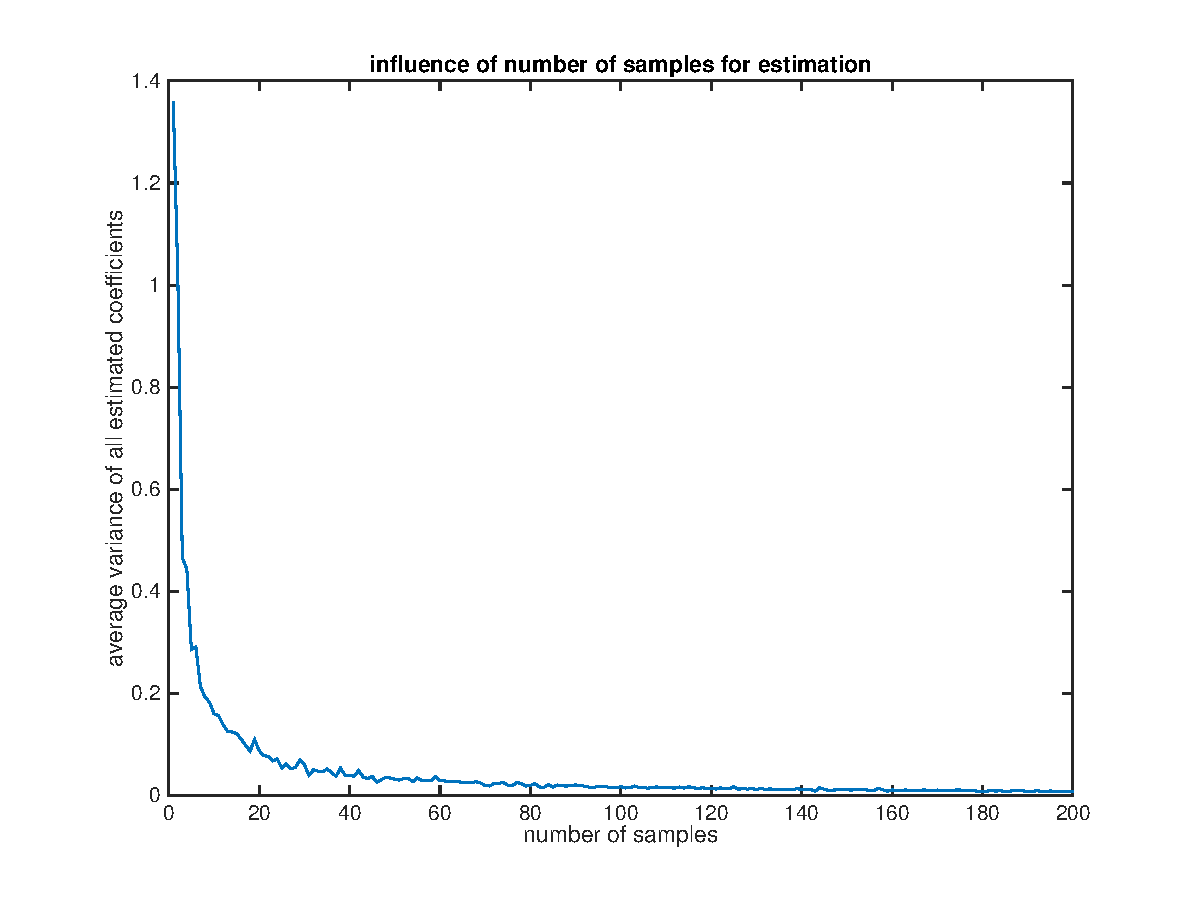
\includegraphics[width=0.5\textwidth]{num_est}
	\caption{average variance of multiple estimations}
	\label{est}
\end{figure}

Note that in the CRT process, we have already computed some subsampled DFT of the signal, in this case, the estimate will come “for free” as part of the identification stage if we keep those subsampled DFTs.

\section{Experimental Evaluation}
For our experiment, we randomly selected k frequencies and set their magnitude to be a randdom number between 0.1 and 1, we lower bounded the coefficient to be over 0.1 because small coefficient can be easily influenced by noise. The coefficients of the rest frequencies are set to be zero. In the influence of noise part of our experiment, our signal is combined with addtive white Gaussian noise, which is parameterized by SNR.

In the runtime experiments, we compared our implementation with the MATLAB built-in FFT function.

\subsection{Runtime vs. Signal Size}
We fixed the signal sparsity to be 15, then computed the runtime of our implementation as the signal size increase, as is shown in Figure (\ref{size}), the FFT algorithm has better performance than ours, as I mentioned above, only the convolution step comsumed us $O(N^2)$ time, thus we can't be faster than FFT, moreover, the MATLAB built-in FFT algorithm is highly optimized on hardware, so the computing speed of it is very fast.
\begin{figure}[htbp]
	\includegraphics[width=0.5\textwidth]{size}
	\caption{runtime increases as signal size increases.}
	\label{size}
\end{figure}

\subsection{Runtime vs. Signal Sparsity}
Here we fixed the signal length to be 512, and computed the runtime as the signal sparsity increase, note that we the signal sparsity increased, the error between original signal and our estimated signal increased, doing more iterations will improve the situation, but it's against the original purpose of the algorithm, to be efficient.
\begin{figure}[htbp]
	\includegraphics[width=0.5\textwidth]{sparsity}
	\caption{runtime increases as signal sparsity increases.}
	\label{sparsity}
\end{figure}
\subsection{Time of Each Part}
We recorded the runtime of our implementation at each stage, it is obvious that the convolution stage take the largest proportion of the whole process, this consistent with our previous derivation. further work must involved on the filter design part.
\begin{figure}[htbp]
	\includegraphics[width=0.5\textwidth]{time}
	\caption{proportion of runtime that each stage take.}
	\label{time}
\end{figure}


\subsection{Influence of Noise}

In order to test the tolerance to noise of our implementation, we combined our test signal with white Gaussian noise of decreasingly small SNR, we compute the error between original spectrum and our estimated spectrum.

\begin{figure}[htbp]
	\includegraphics[width=0.5\textwidth]{influ_noise}
	\caption{error against different level of noise.}
	\label{noise}
\end{figure}

From Figure (\ref{noise}) we can see that when the SNR decrease below $70 dB$, the error increased sharply, in the range of $70 to 100 dB$, the performance is satisfing.

\section{Conclusion and Challenges}
\subsection{Conclusion}
We generated a finite length signal which has certain frequencies randomly appears in frequency domain. Then a permutation method is applied to the time domain to make sure every bin only has one significant frequency. We implemented CRT to find the frequency in each bin and recovered the index based on the mapping relationship from the permutation stage. The rate of correctness is fairly high while an over 70 dB SNR white noise is applied to our generated signal.

We only take a few points from our signal to do the sparse fourier transform in our experiment while the traditional FFT method asks every entry from the signal. But the running time isn’t as fast as the built in FFT algorithm in Matlab. The complexity of filtering process after permutation is $O(N^2)$ which is already slower than the FFT,.Moreover, the built in FFT in Matlab is highly optimized both algorithm-wise and hardware-wise.

An interesting conclusion is that the recovered signal is the phase shifting version of the original signal in time domain while the frequency domain is identical to the original signal. As far as we are concerned that may ascribe to the permutation stage has influence on the statistic of the original signal.

We set a certain sparisity in our experiment but in the real world case usually we don’t know the sparsity. An efficient way is to do a empirical estimation i,e set some empirical sparsity to try, such as image processing empirical conclusion is that 90\% of the points is zero. Another way is to use statistical method to predict the sparsity. The Neyman-Pearson rule is very promising to predict the significant signal components in the receiver array system from our preliminary experiment. 

\subsection{Challenges}
\noindent \textbf{Frequency Leakage} 

	There are frequency leakages in the SFT method since the off-grid frequencies would destroy the sparse nature of the signal. We are expecting applying some widows before permutation to make the leakage into finite bins.
	
\noindent \textbf{Random Permutation}

The signal statistic changes with random permutation. We can’t recover the signal with correct phase in time domain. There is a random phase shifting due to random permutation (figure here). We are expecting to find a permutation scheme that does not affect the statistic of the signal.

\noindent \textbf{Threshold Design}

It is difficult to set a proper threshold to determine the signal from white Gaussian noise. The threshold would significant affect the correct rate in the algorithm. Since the problem might not be convex we are expecting to find some relaxation methods or heuristic algorithm such as Genetic algorithm or Simulated Annealing algorithm to find a local optimal parameter. 

\noindent \textbf{Signal detection difficulty- Difficult to know the exact sparsity in real world cases}

We generate the number of frequencies at the start of the process. i.e the sparsity is defined by us. But in a general real world case for example consider a DOA estimation receiver array. We have to find the sparsity first to make the SFT practical. 
We are expecting to use some statistical methods such as Neyman-Pearson rule to detect the signal. We preliminarily go over some implementations of NP rule in Matlab. We get the threshold in a given false alarm rate from NP rule and the ROC curves from different SNR signals (figure here). We can then detecting the significant part in the time domain of a received signal by this rule and processing SFT. 

\noindent \textbf{Slower}

In our experiment the SFT is slower than FFT. Not only because of that FFT in Matlab is highly optimized but also we find the algorithm from Recent Developments in the Sparse Fourier Transform itself has some steps has relative high complexity than FFT. We apply filter bank after the permutation which makes the complexity become N*N due to the convolution of the permuted signal with the filter bank. We are expecting to use another filter process by Simple and practical algorithm for sparse fourier transform to make SFT become faster. The research team in that paper claimed that their algorithm is much faster than FFT but we don’t implement their algorithm due to limited time.

\noindent \textbf{Prime factorization} 

We have to prime factorize or signal to implement the Chinese Reminder Theory. The big number factorization is a very tough problem nowadays i.e the efficient of big number factorize is fairly low which leads to some encryption algorithms become practical such as RSA encryption algorithm. The basic idea of RSA is to generate big number to encrypt a system that requires over million of years to decrypt (factorize) the password. Back to our algorithm we designed prim pairs in advance to implement the algorithm which is not efficient when the length of signal is enormous. 



\bibliography{refs}
\bibliographystyle{unsrt}
\end{document}


